% Provenance (never printed): cycle 4 SVT, "La planete Terre": the history of
% the Earth read in the rocks, relative dating (superposition, recoupement,
% inclusion, continuite paleontologique), the ages of the Earth, eras and
% periods, the scale of geological time; see sources/book1/PROVENANCE.md.
% Book 1, grade 7, chapter 5.
% Vocabulary guard: owns relative dating / absolute age, the four principles,
% unconformity, era and geological period, the geological time scale. The
% method of radiometric dating is the physics books' and grade 12's: told
% here in two sentences, never defined. Fossils as evidence of evolution are
% the biology books' (one sentence of prose). "Ice age" is grade 8's: not used.
\chapter{Umur Bumi}\label{ch:g7:geological-time}

Pada bulan Juni 1788, ahli geologi Skotlandia James Hutton dan dua orang
temannya, ahli matematika John Playfair dan ahli kimia James Hall,
mengunjungi Siccar Point, sebuah tanjung berbatu yang ``tersapu gundul oleh
\omterm{def:g2:water-on-earth:ocean}{laut}'' di pantai Skotlandia. Di bagian bawah \omterm{def:g3:stones-pebbles-sand:rock}{batuan} itu mereka melihat
lapisan-lapisan kelabu yang berdiri tegak, hampir vertikal. Di atasnya
terdapat lapisan-lapisan batu pasir merah yang landai. Hutton menjelaskan
apa yang telah terjadi: lapisan-lapisan kelabu itu dulu diendapkan secara
mendatar di dasar \omterm{def:g2:water-on-earth:ocean}{laut}, lalu didorong sampai tegak, lalu terkikis, sebelum
\omterm{def:g3:stones-pebbles-sand:sand}{pasir} merah diletakkan di atasnya. Setiap langkah ini memerlukan waktu yang
sangat lama. Kemudian Playfair menulis: ``Pikiran serasa menjadi pening
karena memandang begitu jauh ke dalam jurang waktu.''
% ledger: ncse:siccar-point

\begin{omfigure}
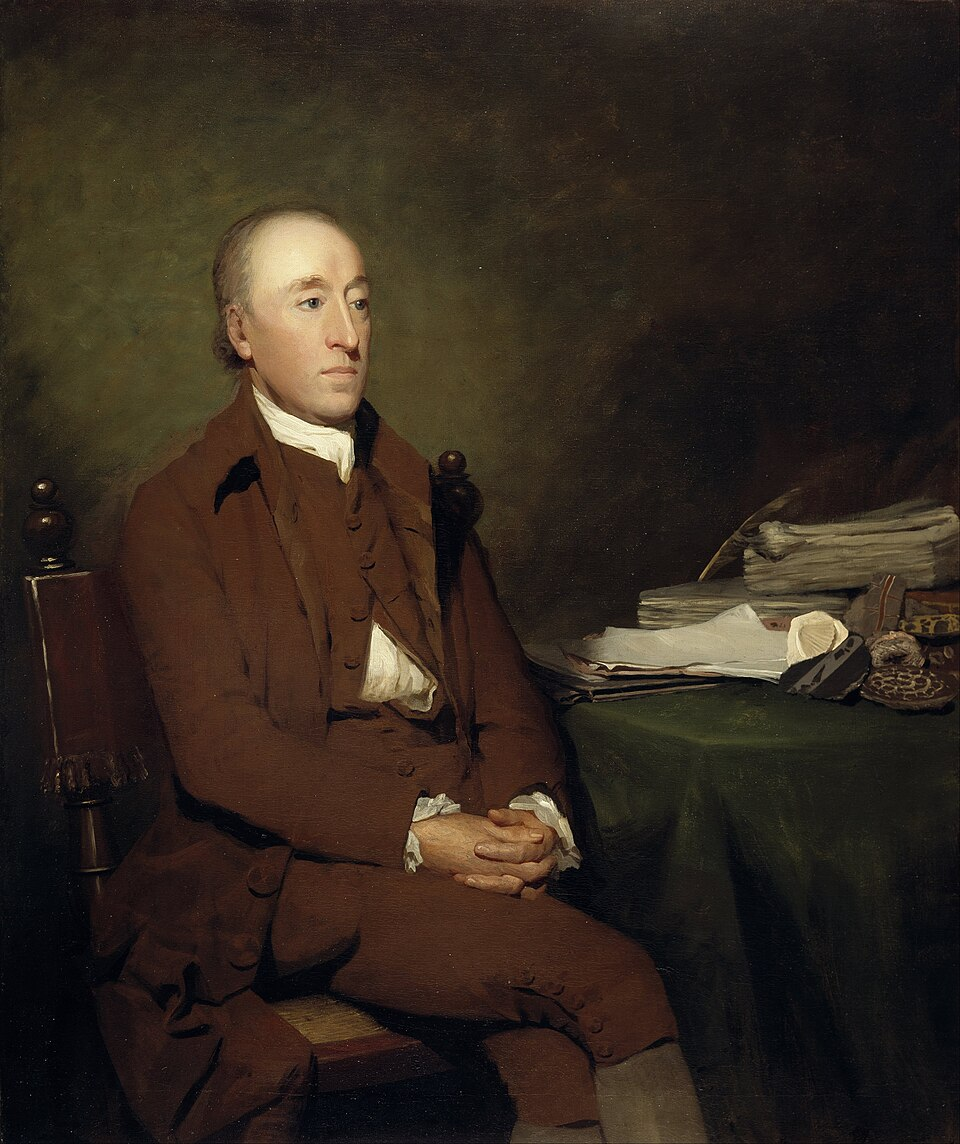
\includegraphics[width=0.3\linewidth]{images/book1/g7-hutton.jpg}

{\small James Hutton (1726--1797), dilukis oleh Henry Raeburn. Hutton
memandang setiap lapisan sebagai suatu rentang waktu, dengan yang paling
tua di bagian bawah di mana pun lapisan-lapisan itu belum terbalik. Potret dalam domain publik, melalui Wikimedia
Commons.}
% ledger: commons:hutton-portrait, usgs:hutton-smith
\label{fig:g7:geological-time:hutton}
\end{omfigure}

Bagaimana kita dapat mengetahui \omterm{def:g3:stones-pebbles-sand:rock}{batuan} mana yang lebih tua daripada \omterm{def:g3:stones-pebbles-sand:rock}{batuan}
lain, tanpa ada tanggal yang tertulis padanya? Berapa umur Bumi? Dan
bagaimana sejarah yang begitu panjang dapat dibayangkan?

\begin{recall}
\omterm{def:g7:sediments-and-fossils:sediment}{Sedimen} mengendap berlapis-lapis, yang satu di atas yang lain, lalu
mengeras menjadi \omterm{def:g6:rocks-and-minerals:rock-families}{batuan sedimen}; \omterm{def:g7:sediments-and-fossils:fossil}{fosil} adalah sisa atau jejak makhluk hidup
yang tersimpan di dalam \omterm{def:g3:stones-pebbles-sand:rock}{batuan} (\cref{ch:g7:sediments-and-fossils}). Yang
disebut \emph{\omterm{def:g7:earthquakes:fault}{sesar}} adalah rekahan pada \omterm{def:g3:stones-pebbles-sand:rock}{batuan} yang di sepanjangnya kedua
sisinya telah bergerak (\cref{ch:g7:earthquakes}). Granit adalah
\emph{\omterm{def:g6:rocks-and-minerals:rock-families}{batuan beku}}: granit terbentuk ketika \omterm{def:g3:stones-pebbles-sand:rock}{batuan} cair mendingin perlahan,
jauh di bawah tanah; sekis adalah \emph{\omterm{def:g6:rocks-and-minerals:rock-families}{batuan metamorf}}, yang diubah oleh
panas dan tekanan; konglomerat adalah \omterm{def:g6:rocks-and-minerals:rock-families}{batuan sedimen} yang terdiri atas
\omterm{def:g3:stones-pebbles-sand:pebble}{kerakal-kerakal} yang tersemen menjadi satu (\cref{ch:g6:rocks-and-minerals}).
\end{recall}

\section{Mana yang lebih dahulu?}

Para ahli sejarah dapat mengurutkan peristiwa-peristiwa bahkan tanpa
tanggalnya. Perang Dunia Pertama terjadi sebelum Perang Dunia Kedua:
namanya sudah mengatakannya. Televisi belum ada di rumah-rumah ketika
Wright bersaudara pertama kali terbang pada tahun 1903, tetapi banyak orang
menonton langkah-langkah pertama di Bulan di televisi pada tahun 1969: jadi
penerbangan itu lebih dahulu, lalu televisi di rumah-rumah, lalu Bulan.
Mengumpulkan petunjuk dan membandingkannya sudah cukup untuk menemukan
urutannya. Untuk hampir seluruh sejarah Bumi sama sekali tidak ada catatan
tertulis, dan para ahli geologi bekerja dengan cara yang sama: mereka
memakai petunjuk-petunjuk yang tersimpan di dalam \omterm{def:g3:stones-pebbles-sand:rock}{batuan}.
% ledger: usgs:events-order

\begin{definition}[Penanggalan relatif dan umur absolut]\label{def:g7:geological-time:relative-dating}
Yang disebut \emph{penanggalan relatif}\index{penanggalan relatif} adalah
pengurutan \omterm{def:g3:stones-pebbles-sand:rock}{batuan} dan peristiwa, dari yang paling tua sampai yang paling
muda, tanpa menyebutkan berapa tahun yang lalu semuanya terjadi: \omterm{def:g3:stones-pebbles-sand:rock}{batuan} ini
lebih tua daripada \omterm{def:g3:stones-pebbles-sand:rock}{batuan} itu. Yang disebut \emph{umur
absolut}\index{umur absolut} adalah umur yang dinyatakan dalam jumlah tahun,
misalnya ``\num{300} juta tahun''.
\end{definition}

\section{Empat prinsip untuk mengurutkan batuan}

Empat prinsip sederhana melakukan sebagian besar pekerjaan \omterm{def:g7:geological-time:relative-dating}{penanggalan
relatif}. Prinsip-prinsip itu digambarkan di bawah ini, pada empat tebing khayalan. Prinsip yang pertama dinyatakan oleh Nicolas Steno pada tahun 1669; Hutton membangun di atasnya pada akhir abad kedelapan belas.
% ledger: usgs:hutton-smith, og:stratigraphy-principles

\begin{omfigure}
\tikzset{
  trilo/.pic={\fill[black!65] (0,0) ellipse (0.13 and 0.085);
              \draw[white, line width=0.3pt] (-0.11,0.028) -- (0.11,0.028) (-0.11,-0.028) -- (0.11,-0.028);},
  ammo/.pic={\draw[black!75, line width=0.45pt] (0,0) circle (0.1) (0,0) circle (0.062) (0,0) circle (0.028);}
}
\begin{minipage}[t]{0.49\linewidth}\centering
\begin{tikzpicture}[font=\footnotesize]
  \fill[lith sandstone] (0,0) rectangle (4.4,0.6);
  \fill[lith shale] (0,0.6) rectangle (4.4,1.2);
  \fill[lith limestone] (0,1.2) rectangle (4.4,1.8);
  \fill[lith sandstone] (0,1.8) rectangle (4.4,2.4);
  \foreach \k in {1,2,3,4} \node[fill=white, inner sep=1pt] at (0.35,0.6*\k-0.3) {\k};
  \draw (0,0) rectangle (4.4,2.4);
  \foreach \y in {0.6,1.2,1.8} \draw[contact] (0,\y) -- (4.4,\y);
  \draw[-{Stealth}, line width=0.8pt] (4.75,0.1) -- (4.75,2.3);
  \node[anchor=west] at (4.85,2.2) {paling muda};
  \node[anchor=west] at (4.85,0.2) {paling tua};
\end{tikzpicture}

{\small (a) Superposisi: lapisan 1 terbentuk paling dahulu, lapisan 4 paling akhir.}
\end{minipage}\hfill
\begin{minipage}[t]{0.49\linewidth}\centering
\begin{tikzpicture}[font=\footnotesize]
  % left block, below the fault
  \begin{scope}
    \clip (0,0) -- (3.75,0) -- (3.25,2.4) -- (0,2.4) -- cycle;
    \fill[lith sandstone] (0,0) rectangle (5,0.6);
    \fill[lith shale] (0,0.6) rectangle (5,1.2);
    \fill[lith limestone] (0,1.2) rectangle (5,1.8);
    \fill[lith granite] (1.2,0) -- (1.85,0) -- (1.75,0.9) -- (1.9,1.8) -- (1.15,1.8) -- (1.3,0.9) -- cycle;
    \fill[lith sandstone] (0,1.8) rectangle (5,2.4);
    \foreach \y in {0.6,1.2} {\draw[contact] (0,\y) -- (1.25,\y); \draw[contact] (1.8,\y) -- (5,\y);}
    \draw[contact] (1.2,0) -- (1.3,0.9) -- (1.15,1.8) (1.85,0) -- (1.75,0.9) -- (1.9,1.8);
    \draw[contact] (0,1.8) -- (5,1.8);
  \end{scope}
  % right block, moved down along the fault
  \begin{scope}
    \clip (3.75,0) -- (5,0) -- (5,2.05) -- (3.32,2.05) -- cycle;
    \fill[lith sandstone] (3,-0.35) rectangle (5,0.25);
    \fill[lith shale] (3,0.25) rectangle (5,0.85);
    \fill[lith limestone] (3,0.85) rectangle (5,1.45);
    \fill[lith sandstone] (3,1.45) rectangle (5,2.05);
    \foreach \y in {0.25,0.85,1.45} \draw[contact] (3,\y) -- (5,\y);
  \end{scope}
  \draw (0,0) -- (5,0) -- (5,2.05) -- (3.32,2.05) (3.25,2.4) -- (0,2.4) -- (0,0);
  \draw[fault] (3.75,0) -- (3.25,2.4);
  \node[anchor=south, fill=white, inner sep=1pt] at (1.5,2.45) {granit};
  \draw[black!70] (1.5,2.45) -- (1.52,1.6);
  \node[anchor=south] at (4.2,2.45) {sesar};
  \draw[black!70] (4.0,2.45) -- (3.4,1.75);
\end{tikzpicture}

{\small (b) Potong-memotong: granit itu lebih muda daripada ketiga lapisan
yang dipotongnya, lebih tua daripada lapisan teratas; \omterm{def:g7:earthquakes:fault}{sesar}, yang
mematahkan semuanya, adalah yang paling muda.}
\end{minipage}

\bigskip
\begin{minipage}[t]{0.49\linewidth}\centering
\begin{tikzpicture}[font=\footnotesize]
  \fill[lith granite] (0,0) -- (4.4,0) -- (4.4,1.05) .. controls (3.4,0.95) and (2.6,1.2) .. (1.6,1.0) .. controls (0.9,0.88) and (0.4,1.1) .. (0,1.0) -- cycle;
  \fill[lith conglomerate] (0,2.4) -- (4.4,2.4) -- (4.4,1.05) .. controls (3.4,0.95) and (2.6,1.2) .. (1.6,1.0) .. controls (0.9,0.88) and (0.4,1.1) .. (0,1.0) -- cycle;
  \foreach \x/\y/\a/\b in {0.5/1.35/0.2/0.12, 1.3/1.25/0.16/0.1, 2.1/1.45/0.22/0.13, 2.9/1.3/0.17/0.11, 3.7/1.4/0.2/0.12, 0.9/1.8/0.15/0.1, 2.5/1.95/0.17/0.1, 3.4/1.85/0.14/0.09}
    \filldraw[fill=omLithGranite, draw=black!70, line width=0.3pt] (\x,\y) ellipse [x radius=\a, y radius=\b];
  \draw[unconformity] (0,1.0) .. controls (0.4,1.1) and (0.9,0.88) .. (1.6,1.0) .. controls (2.6,1.2) and (3.4,0.95) .. (4.4,1.05);
  \draw (0,0) rectangle (4.4,2.4);
  \node[fill=white, inner sep=1pt] at (2.2,0.45) {granit};
  \node[anchor=west] at (4.5,1.7) {konglomerat};
  \node[anchor=west, align=left] at (4.5,1.15) {kerakal\\granit};
  \draw[black!70] (4.5,1.15) -- (3.85,1.4);
\end{tikzpicture}

{\small (c) Inklusi: \omterm{def:g3:stones-pebbles-sand:pebble}{kerakal-kerakal} granit itu lebih tua daripada
konglomerat yang mengandungnya.}
\end{minipage}\hfill
\begin{minipage}[t]{0.49\linewidth}\centering
\begin{tikzpicture}[font=\footnotesize]
  % place A
  \fill[lith shale] (0,0) rectangle (1.3,0.8);
  \fill[lith limestone] (0,0.8) rectangle (1.3,1.6);
  \fill[lith sandstone] (0,1.6) rectangle (1.3,2.4);
  \draw (0,0) rectangle (1.3,2.4); \draw[contact] (0,0.8) -- (1.3,0.8) (0,1.6) -- (1.3,1.6);
  \foreach \x in {0.3,0.65,1.0} {\pic at (\x,0.4) {trilo}; \pic at (\x,1.2) {ammo};}
  \node[anchor=south] at (0.65,2.45) {tempat A};
  % place B
  \fill[lith sandstone] (3.6,0.4) rectangle (4.9,1.0);
  \fill[lith shale] (3.6,1.0) rectangle (4.9,2.0);
  \fill[lith limestone] (3.6,0) rectangle (4.9,0.4);
  \draw (3.6,0) rectangle (4.9,2.0); \draw[contact] (3.6,0.4) -- (4.9,0.4) (3.6,1.0) -- (4.9,1.0);
  \foreach \x in {3.9,4.25,4.6} {\pic at (\x,0.7) {trilo}; \pic at (\x,1.5) {ammo};}
  \node[anchor=south] at (4.25,2.45) {tempat B};
  \draw[dashed, black!70] (1.3,0.8) -- (3.6,1.0) (1.3,0) -- (3.6,0.4) (1.3,1.6) -- (3.6,2.0);
  \pic at (2.15,-0.3) {trilo}; \node[anchor=west] at (2.3,-0.3) {trilobit};
  \pic at (2.15,2.3) {ammo}; \node[anchor=west] at (2.3,2.3) {amonit};
\end{tikzpicture}

{\small (d) Suksesi \omterm{def:g7:sediments-and-fossils:fossil}{fosil}: lapisan-lapisan dengan \omterm{def:g7:sediments-and-fossils:fossil}{fosil} yang sama berumur
sama, walaupun \omterm{def:g3:stones-pebbles-sand:rock}{batuannya} berbeda.}
\end{minipage}

\medskip
{\small Empat prinsip \omterm{def:g7:geological-time:relative-dating}{penanggalan relatif}, pada empat tebing
khayalan.}
% ledger: usgs:hutton-smith, usgs:cross-cutting, nps:cross-cutting, eli:relative-dating, usgs:fossil-succession
\label{fig:g7:geological-time:principles}
\end{omfigure}

\begin{definition}[Prinsip superposisi]\label{def:g7:geological-time:superposition}
Yang disebut \emph{prinsip superposisi}\index{superposisi, prinsip} adalah
prinsip berikut: dalam setumpuk \omterm{def:g7:sediments-and-fossils:layer}{lapisan sedimen} yang belum terbalik, setiap
lapisan lebih muda daripada lapisan di bawahnya dan lebih tua daripada
lapisan di atasnya. Lapisan yang paling tua berada di bagian bawah, yang
paling muda di bagian atas.
\end{definition}
% ledger: usgs:hutton-smith, eli:relative-dating

\begin{definition}[Prinsip hubungan potong-memotong]\label{def:g7:geological-time:cross-cutting}
Yang disebut \emph{prinsip hubungan potong-memotong}\index{hubungan potong-memotong, prinsip} adalah prinsip berikut: \omterm{def:g3:stones-pebbles-sand:rock}{batuan} atau struktur yang memotong
\omterm{def:g3:stones-pebbles-sand:rock}{batuan} lain lebih muda daripada \omterm{def:g3:stones-pebbles-sand:rock}{batuan} yang dipotongnya. Massa granit yang
memotong lapisan-lapisan, \omterm{def:g7:earthquakes:fault}{sesar} yang mematahkannya, dan permukaan \omterm{def:g5:water-shapes-the-land:erosion}{erosi}
yang mengikisnya semuanya lebih muda daripada lapisan-lapisan itu.
\end{definition}
% ledger: usgs:cross-cutting, nps:cross-cutting, eli:relative-dating

\begin{definition}[Prinsip inklusi]\label{def:g7:geological-time:inclusion}
Yang disebut \emph{prinsip inklusi}\index{inklusi, prinsip} adalah prinsip
berikut: kepingan suatu \omterm{def:g3:stones-pebbles-sand:rock}{batuan} yang ditemukan di dalam \omterm{def:g3:stones-pebbles-sand:rock}{batuan} lain lebih
tua daripada \omterm{def:g3:stones-pebbles-sand:rock}{batuan} yang mengandungnya. \omterm{def:g3:stones-pebbles-sand:pebble}{Kerakal-kerakal} sebuah konglomerat
sudah ada sebelum konglomerat itu terbentuk di sekelilingnya.
\end{definition}
% ledger: eli:relative-dating

\begin{definition}[Prinsip suksesi fosil]\label{def:g7:geological-time:fossil-succession}
Yang disebut \emph{prinsip suksesi fosil}\index{suksesi fosil, prinsip} adalah prinsip berikut: jenis-jenis hewan dan tumbuhan yang ditemukan sebagai
\omterm{def:g7:sediments-and-fossils:fossil}{fosil} berubah dari lapisan yang lebih tua ke lapisan yang lebih muda, selalu
dengan urutan yang sama. \omterm{def:g3:stones-pebbles-sand:rock}{Batuan} yang mengandung jenis-jenis \omterm{def:g7:sediments-and-fossils:fossil}{fosil} yang sama
berumur sama, bahkan jika letaknya berjauhan.
\end{definition}
% ledger: usgs:fossil-succession


\omterm{def:g7:geological-time:superposition}{Prinsip superposisi} hanya berlaku untuk lapisan-lapisan yang belum
terbalik: di beberapa tempat, pembentukan \omterm{def:g4:world-physical-map:range}{pegunungan} telah melipat setumpuk
lapisan begitu kuat sehingga tumpukan itu terletak terbalik. Para ahli
geologi lalu mencari petunjuk yang menunjukkan sisi mana yang di atas ketika
lapisan-lapisan itu terbentuk --- jejak kaki dan gelembur gelombang,
misalnya, terdapat pada permukaan atas sebuah lapisan. \omterm{def:g7:geological-time:fossil-succession}{Prinsip suksesi
fosil} berlaku karena kehidupan di Bumi telah berubah sepanjang waktu:
sebagian besar \omterm{def:g7:sediments-and-fossils:fossil}{fosil} berasal dari spesies yang sudah tidak hidup di mana
pun. Mengapa kehidupan berubah diceritakan dalam buku-buku biologi.
% ledger: eli:relative-dating, usgs:fossil-succession, nps:ripple-marks

\begin{history}[William Smith, pembangun kanal]
Antara tahun 1785 dan 1800, ketika Hutton bekerja di Skotlandia, William
Smith, seorang insinyur Inggris yang membangun kanal-kanal, mengumpulkan
\omterm{def:g7:sediments-and-fossils:fossil}{fosil} cangkang dari batu kapur dan serpih yang digalinya. Ia mendapati
bahwa setiap lapisan mengandung \omterm{def:g7:sediments-and-fossils:fossil}{fosilnya} sendiri, yang berbeda dari \omterm{def:g7:sediments-and-fossils:fossil}{fosil}
lapisan di atas dan di bawahnya. Dengan memakai \omterm{def:g7:sediments-and-fossils:fossil}{fosil-fosil} ini sebagai
penanda, ia dapat mengenali lapisan yang sama di mana pun lapisan itu
muncul, dan ia menggambar beberapa \omterm{def:g2:drawing-to-map:map}{peta} geologi pertama untuk daerah yang
luas.
\end{history}
% ledger: usgs:hutton-smith

\section{Celah dalam catatan}

Di Siccar Point, lapisan-lapisan kelabu dan batu pasir merah itu tidak
terbentuk berturut-turut. Di antara keduanya, lapisan-lapisan kelabu itu
dimiringkan dan diangkat, lalu terkikis untuk waktu yang sangat lama, dan
tidak ada lapisan dari masa itu yang tersimpan. Permukaan di antara kedua
kelompok \omterm{def:g3:stones-pebbles-sand:rock}{batuan} itu adalah sebuah celah dalam catatan.

\begin{definition}[Ketidakselarasan]\label{def:g7:geological-time:unconformity}
Yang disebut \emph{ketidakselarasan}\index{ketidakselarasan} adalah permukaan
\omterm{def:g5:water-shapes-the-land:erosion}{erosi} di antara dua kelompok \omterm{def:g3:stones-pebbles-sand:rock}{batuan} yang terbentuk pada waktu yang sangat
berbeda: \omterm{def:g3:stones-pebbles-sand:rock}{batuan} yang lebih tua terkikis sebelum \omterm{def:g3:stones-pebbles-sand:rock}{batuan} yang lebih muda
diendapkan di atasnya. Ketidakselarasan menandai waktu yang lama yang tidak
meninggalkan satu lapisan pun.
\end{definition}
% ledger: ncse:siccar-point, eli:relative-dating

\begin{omfigure}
\begin{tikzpicture}[font=\footnotesize, x=1cm, y=1cm]
  \def\stripes#1#2#3{% x0, width, top: vertical layers
    \foreach \i in {0,...,7} {
      \pgfmathsetmacro{\xa}{#1+\i*#2/8}
      \pgfmathsetmacro{\xb}{#1+(\i+1)*#2/8}
      \ifodd\i\def\lithc{omLithSchist}\else\def\lithc{omLithShale}\fi
      \fill[\lithc] (\xa,0) rectangle (\xb,#3);
      \draw[black!55, line width=0.3pt] (\xa,0) -- (\xa,#3);
    }}
  % 1: flat layers under the sea
  \fill[omSea!70] (0,1.6) rectangle (3.4,2.4);
  \foreach \k in {0,...,3} {
    \ifodd\k\def\lithc{omLithSchist}\else\def\lithc{omLithShale}\fi
    \fill[\lithc] (0,0.4*\k) rectangle (3.4,0.4*\k+0.4);
    \draw[black!55, line width=0.3pt] (0,0.4*\k) -- (3.4,0.4*\k);
  }
  \draw (0,0) rectangle (3.4,2.4);
  \node[anchor=north, align=center] at (1.7,-0.1) {1. Lapisan diendapkan\\mendatar di laut};
  % 2: pushed up on end
  \begin{scope}[xshift=3.9cm]
    \begin{scope}
      \clip (0,0) -- (3.4,0) -- (3.4,1.7) -- (2.6,2.2) -- (1.6,1.75) -- (0.9,2.3) -- (0,1.8) -- cycle;
      \stripes{0}{3.4}{2.4}
    \end{scope}
    \draw (0,1.8) -- (0.9,2.3) -- (1.6,1.75) -- (2.6,2.2) -- (3.4,1.7);
    \draw (0,1.8) -- (0,0) -- (3.4,0) -- (3.4,1.7);
    \node[anchor=north, align=center] at (1.7,-0.1) {2. Didorong sampai tegak,\\terangkat di atas laut};
  \end{scope}
  % 3: worn flat
  \begin{scope}[xshift=7.8cm]
    \stripes{0}{3.4}{1.3}
    \draw[unconformity] (0,1.3) -- (3.4,1.3);
    \draw (0,1.3) -- (0,0) -- (3.4,0) -- (3.4,1.3);
    \node[anchor=north, align=center] at (1.7,-0.1) {3. Terkikis\\untuk waktu lama};
  \end{scope}
  % 4: new layers on top
  \begin{scope}[xshift=11.7cm]
    \stripes{0}{3.4}{1.3}
    \fill[om lith={red!22}{om sand}] (0,1.3) rectangle (3.4,1.85);
    \fill[om lith={red!30}{om sand}] (0,1.85) rectangle (3.4,2.4);
    \draw[contact] (0,1.85) -- (3.4,1.85);
    \draw[unconformity, line width=0.9pt] (0,1.3) -- (3.4,1.3);
    \draw (0,0) rectangle (3.4,2.4);
    \node[anchor=north, align=center] at (1.7,-0.1) {4. Lapisan baru di atasnya:\\sebuah ketidakselarasan};
  \end{scope}
  \foreach \x in {3.45,7.35,11.25} \draw[-{Stealth}, line width=0.7pt] (\x,1.2) -- (\x+0.4,1.2);
\end{tikzpicture}

{\small Bagaimana \omterm{def:g7:geological-time:unconformity}{ketidakselarasan} seperti yang ada di Siccar Point
terbentuk. Garis yang bergelombang adalah \omterm{def:g7:geological-time:unconformity}{ketidakselarasan} itu: waktu yang
lama pada langkah 2 dan 3 tidak meninggalkan lapisan apa pun.}
% ledger: ncse:siccar-point
\label{fig:g7:geological-time:unconformity}
\end{omfigure}

\section{Membaca sejarah sebuah wilayah}

Penampang menunjukkan \omterm{def:g3:stones-pebbles-sand:rock}{batuan} sebagaimana akan tampak pada sebuah irisan
yang lurus ke bawah ke dalam tanah. Keempat prinsip itu mengubahnya menjadi
sebuah cerita.

\begin{method}[Mengurutkan peristiwa-peristiwa pada sebuah penampang]\label{met:g7:geological-time:ordering}
\begin{enumerate}
  \item Temukan \omterm{def:g3:stones-pebbles-sand:rock}{batuan} yang paling tua: \omterm{def:g3:stones-pebbles-sand:rock}{batuan} yang dipotong oleh semua yang
        lain, atau yang terletak di bagian bawah tumpukan.
  \item Temukan setiap \omterm{def:g3:stones-pebbles-sand:rock}{batuan} atau struktur yang memotong yang lain
        (granit, \omterm{def:g7:earthquakes:fault}{sesar}, permukaan \omterm{def:g5:water-shapes-the-land:erosion}{erosi}): \omterm{def:g3:stones-pebbles-sand:rock}{batuan} atau struktur itu lebih
        muda daripada semua yang dipotongnya.
  \item Bacalah lapisan-lapisan dari bawah ke atas (superposisi), dan
        carilah \omterm{def:g7:geological-time:unconformity}{ketidakselarasan}, tempat waktu hilang.
  \item Lapisan diendapkan secara mendatar: jika lapisan itu miring atau
        terlipat, pelipatan itu terjadi sesudahnya.
  \item Tuliskan peristiwa-peristiwa itu secara berurutan, dari yang
        paling tua sampai yang paling muda, dengan petunjuk untuk
        masing-masing.
\end{enumerate}
\end{method}
% ledger: eli:relative-dating, usgs:cross-cutting, nps:cross-cutting

\begin{omfigure}
\begin{tikzpicture}
\begin{axis}[x=1.4cm, y=0.007cm, xmin=0, xmax=10, ymin=-500, ymax=300,
  axis on top, tick label style={font=\scriptsize}, label style={font=\small},
  xlabel={jarak ke timur dari E (km)}, ylabel={ketinggian (m)},
  ytick={-400,-200,0,200}, clip mode=individual]
\addplot[lith schist, draw=black, line width=0.3pt, even odd rule] table {figdata/out/grade-7-varden_history-unit-schist.dat};
\addplot[lith granite, draw=black, line width=0.3pt, even odd rule] table {figdata/out/grade-7-varden_history-unit-granite.dat};
\addplot[om lith={icsTriassic!35}{om sand}, draw=black, line width=0.3pt, even odd rule] table {figdata/out/grade-7-varden_history-unit-sandstone.dat};
\addplot[om lith={icsJurassic!40}{om limestone}, draw=black, line width=0.3pt, even odd rule] table {figdata/out/grade-7-varden_history-unit-limestone.dat};
\addplot[om lith={icsJurassic!15}{om shale}, draw=black, line width=0.3pt, even odd rule] table {figdata/out/grade-7-varden_history-unit-shale.dat};
\addplot[om lith={icsCretaceous!35}{om limestone}, draw=black, line width=0.3pt, even odd rule] table {figdata/out/grade-7-varden_history-unit-chalk.dat};
\addplot[lith alluvium, draw=black, line width=0.3pt, even odd rule] table {figdata/out/grade-7-varden_history-unit-alluvium.dat};
\addplot[omThm, line width=1.3pt] table {figdata/out/grade-7-varden_history-base.dat};
\addplot[black, line width=0.8pt] table {figdata/out/grade-7-varden_history-ground.dat};
\addplot[fault, line width=1.3pt] table {figdata/out/grade-7-varden_history-fault.dat};
\node[font=\small, above right] at (axis cs:0,300) {E (barat)};
\node[font=\small, above left] at (axis cs:10,300) {F (timur)};
\end{axis}
\end{tikzpicture}

\smallskip
{\small\setlength{\tabcolsep}{4pt}
\begin{tabular}{@{}llll@{}}
\tikz\fill[lith schist, draw=black] (0,0) rectangle (0.5,0.3); sekis &
\tikz\fill[lith granite, draw=black] (0,0) rectangle (0.5,0.3); granit &
\tikz\fill[om lith={icsTriassic!35}{om sand}, draw=black] (0,0) rectangle (0.5,0.3); batu pasir &
\tikz\fill[om lith={icsJurassic!40}{om limestone}, draw=black] (0,0) rectangle (0.5,0.3); batu kapur \\
\tikz\fill[om lith={icsJurassic!15}{om shale}, draw=black] (0,0) rectangle (0.5,0.3); serpih &
\tikz\fill[om lith={icsCretaceous!35}{om limestone}, draw=black] (0,0) rectangle (0.5,0.3); kapur &
\tikz\fill[lith alluvium, draw=black] (0,0) rectangle (0.5,0.3); \omterm{def:g3:stones-pebbles-sand:sand}{pasir} \omterm{def:g1:landscapes-around-us:water}{sungai} &
\tikz\draw[omThm, line width=1.3pt] (0,0.15) -- (0.5,0.15); alas batu pasir \\
\end{tabular}}

\smallskip
{\small Penampang E--F, dari barat (E) ke timur (F) melintasi bagian tengah
Perbukitan Varden, wilayah rekaan dalam seri ini, melalui granitnya. Garis
hitam yang tebal adalah \omterm{def:g7:earthquakes:fault}{sesar}. \omterm{def:g4:world-physical-map:altitude}{Ketinggiannya} direntangkan 5 kali
dibandingkan dengan jaraknya, agar lapisan-lapisannya lebih mudah dilihat.}
% ledger: (invented region: figdata/shared/region.py, section E--F by figdata/grade-7/varden_history.py)
\label{fig:g7:geological-time:section}
\end{omfigure}

\begin{example}[Sejarah Perbukitan Varden]\label{ex:g7:geological-time:varden}
Terapkan metode itu pada penampang E--F.
\begin{enumerate}
  \item Sekis dipotong oleh granit dan terletak di bawah semua lapisan:
        sekis adalah \omterm{def:g3:stones-pebbles-sand:rock}{batuan} yang paling tua.
  \item Granit memotong sekis (potong-memotong), jadi granit lebih muda.
        Granit tidak memotong satu pun lapisan di atasnya: granit lebih tua
        daripada batu pasir.
  \item Granit mendingin jauh di bawah tanah, tetapi alas batu pasir, yang
        terletak di atas sekis, mencapai puncak granit: \omterm{def:g3:stones-pebbles-sand:rock}{batuan} yang
        menutupi keduanya terkikis sebelum \omterm{def:g3:stones-pebbles-sand:sand}{pasir} datang. Alas batu pasir
        adalah sebuah \omterm{def:g7:geological-time:unconformity}{ketidakselarasan}.
  \item Batu pasir, batu kapur, serpih, dan kapur diendapkan dengan urutan
        itu (superposisi).
  \item Lapisan-lapisan itu diendapkan secara mendatar, tetapi kini
        lapisan-lapisan itu terlipat, melengkung ke atas di atas granit dan
        melengkung ke bawah lebih jauh ke timur: pelipatan itu terjadi
        sesudah kapur.
  \item \omterm{def:g7:earthquakes:fault}{Sesar} mematahkan semua lapisan yang terlipat: \omterm{def:g7:earthquakes:fault}{sesar} itu lebih muda
        daripada pelipatan.
  \item Permukaan tanah masa kini memotong segalanya, dan \omterm{def:g3:stones-pebbles-sand:sand}{pasir} \omterm{def:g1:landscapes-around-us:water}{sungai}
        terletak di atasnya: \omterm{def:g5:water-shapes-the-land:erosion}{erosi} dan \omterm{def:g1:landscapes-around-us:water}{sungai-sungai} adalah peristiwa yang
        paling baru.
\end{enumerate}
Sejarahnya, yang paling tua lebih dahulu: sekis; granit; \omterm{def:g5:water-shapes-the-land:erosion}{erosi}; keempat
lapisan; pelipatan; \omterm{def:g7:earthquakes:fault}{sesar}; \omterm{def:g5:water-shapes-the-land:erosion}{erosi} dan \omterm{def:g3:stones-pebbles-sand:sand}{pasir} \omterm{def:g1:landscapes-around-us:water}{sungai} masa kini.
% ledger: (invented region: figdata/grade-7/varden_history.py main table)
\end{example}

\omterm{def:g7:geological-time:relative-dating}{Penanggalan relatif} memberikan urutan peristiwa, tetapi tidak memberikan
tanggalnya ataupun berapa lama setiap peristiwa berlangsung: metode itu
mengatakan bahwa \omterm{def:g7:earthquakes:fault}{sesar} lebih muda daripada kapur, tetapi tidak berapa tahun
lebih muda.

\section{Era dan zaman}

Suksesi \omterm{def:g7:sediments-and-fossils:fossil}{fosil} memungkinkan para ahli geologi mencocokkan lapisan-lapisan di
seluruh dunia. Dengan menggabungkan pengamatan mereka, mereka membagi
sejarah Bumi menjadi rentang-rentang waktu, sama seperti para ahli sejarah
berbicara tentang abad-abad dan masa pemerintahan raja-raja.
% ledger: usgs:hutton-smith, usgs:fossil-succession

\begin{omfigure}
\begin{tikzpicture}[font=\footnotesize]
\begin{axis}[name=long, x dir=reverse, xmin=0, xmax=4600, ymin=0, ymax=1,
  width=14.3cm, height=1.7cm, scale only axis, axis y line=none, axis x line*=bottom,
  xtick={4500,4000,3000,2000,1000}, tick label style={font=\scriptsize}, clip=false]
  \pgfplotsinvokeforeach{Hadean,Archean,Proterozoic,Phanerozoic}{
    \addplot[fill=ics#1, draw=black!70, line width=0.3pt] table {figdata/out/grade-7-time_scale-bar-#1.dat};}
  \node[anchor=center, font=\scriptsize, fill=white, fill opacity=0.85, text opacity=1, inner sep=1pt] at (axis cs:4299,0.5) {Hadean};
  \node[anchor=center, font=\scriptsize, fill=white, fill opacity=0.85, text opacity=1, inner sep=1pt] at (axis cs:3265.5,0.5) {Arkean};
  \node[anchor=center, font=\scriptsize, fill=white, fill opacity=0.85, text opacity=1, inner sep=1pt] at (axis cs:1519.4,0.5) {Proterozoikum};
  \node[anchor=center, font=\scriptsize, align=center, fill=white, fill opacity=0.85, text opacity=1, inner sep=1pt] at (axis cs:269.4,0.5) {Fanero-\\zoikum};
  \coordinate (z1) at (axis cs:538.8,0);
  \coordinate (z2) at (axis cs:0,0);
\end{axis}
\begin{axis}[at={(long.south west)}, anchor=north west, yshift=-1.3cm,
  x dir=reverse, xmin=0, xmax=540, ymin=0, ymax=3.2,
  width=14.3cm, height=3.6cm, scale only axis, axis y line=none, axis x line*=bottom,
  xtick={500,400,300,200,100,0}, tick label style={font=\scriptsize},
  xlabel={juta tahun yang lalu}, label style={font=\small}, clip=false]
  \pgfplotsinvokeforeach{Paleozoic,Mesozoic,Cenozoic}{
    \addplot[fill=ics#1, draw=black!70, line width=0.3pt] table[x=age, y expr=2.4+0.8*\thisrow{y}] {figdata/out/grade-7-time_scale-bar-#1.dat};}
  \pgfplotsinvokeforeach{Cambrian,Ordovician,Silurian,Devonian,Carboniferous,Permian,Triassic,Jurassic,Cretaceous,Paleogene,Neogene,Quaternary}{
    \addplot[fill=ics#1, draw=black!70, line width=0.3pt] table[x=age, y expr=2.4*\thisrow{y}] {figdata/out/grade-7-time_scale-bar-#1.dat};}
  \node[anchor=center, font=\footnotesize\bfseries, fill=white, fill opacity=0.85, text opacity=1, inner sep=1pt] at (axis cs:395.351,2.8) {Paleozoikum};
  \node[anchor=center, font=\footnotesize\bfseries, fill=white, fill opacity=0.85, text opacity=1, inner sep=1pt] at (axis cs:158.951,2.8) {Mesozoikum};
  \node[anchor=center, font=\scriptsize\bfseries, fill=white, fill opacity=0.85, text opacity=1, inner sep=1pt] at (axis cs:33,2.8) {Kenozoikum};
  \node[anchor=center, rotate=90, font=\scriptsize, fill=white, fill opacity=0.85, text opacity=1, inner sep=1pt] at (axis cs:512.825,1.2) {Kambrium};
  \node[anchor=center, rotate=90, font=\scriptsize, fill=white, fill opacity=0.85, text opacity=1, inner sep=1pt] at (axis cs:464.975,1.2) {Ordovisium};
  \node[anchor=center, rotate=90, font=\scriptsize, fill=white, fill opacity=0.85, text opacity=1, inner sep=1pt] at (axis cs:431.36,1.2) {Silur};
  \node[anchor=center, rotate=90, font=\scriptsize, fill=white, fill opacity=0.85, text opacity=1, inner sep=1pt] at (axis cs:389.24,1.2) {Devon};
  \node[anchor=center, rotate=90, font=\scriptsize, fill=white, fill opacity=0.85, text opacity=1, inner sep=1pt] at (axis cs:328.88,1.2) {Karbon};
  \node[anchor=center, rotate=90, font=\scriptsize, fill=white, fill opacity=0.85, text opacity=1, inner sep=1pt] at (axis cs:275.401,1.2) {Perm};
  \node[anchor=center, rotate=90, font=\scriptsize, fill=white, fill opacity=0.85, text opacity=1, inner sep=1pt] at (axis cs:226.651,1.2) {Trias};
  \node[anchor=center, rotate=90, font=\scriptsize, fill=white, fill opacity=0.85, text opacity=1, inner sep=1pt] at (axis cs:172.25,1.2) {Jura};
  \node[anchor=center, rotate=90, font=\scriptsize, fill=white, fill opacity=0.85, text opacity=1, inner sep=1pt] at (axis cs:104.55,1.2) {Kapur};
  \node[anchor=center, rotate=90, font=\scriptsize, fill=white, fill opacity=0.85, text opacity=1, inner sep=1pt] at (axis cs:44.52,1.2) {Paleogen};
  \node[anchor=center, rotate=90, font=\scriptsize, fill=white, fill opacity=0.85, text opacity=1, inner sep=1pt] at (axis cs:12.81,1.2) {Neogen};
  \node[anchor=west, xshift=3pt, font=\scriptsize] at (axis cs:1.29,1.2) {Kuarter};
  \coordinate (w1) at (axis cs:540,3.2);
  \coordinate (w2) at (axis cs:0,3.2);
\end{axis}
\draw[dashed, black!60] (z1) -- ++(0,-0.5) -- (w1) (z2) -- (w2);
\end{tikzpicture}

{\small Skala waktu geologi, dengan warna-warna bagan internasional. Atas:
seluruh sejarah Bumi. Bawah: bagian terakhirnya, Fanerozoikum, yang
direntangkan: ketiga \omterm{def:g7:geological-time:era-period}{eranya}, dan kedua belas \omterm{def:g7:geological-time:era-period}{zaman geologinya}. Umur dalam
juta tahun sebelum masa kini.}
% ledger: ics:base.Hadean, ics:base.Archean, ics:base.Proterozoic, ics:base.Paleozoic, ics:base.Mesozoic, ics:base.Cenozoic, ics:colour.Hadean (figdata/grade-7/time_scale.py reads every ics base and colour row of the shared ledger)
\label{fig:g7:geological-time:scale}
\end{omfigure}

\begin{definition}[Era dan zaman geologi]\label{def:g7:geological-time:era-period}
Yang disebut \emph{era}\index{era} adalah rentang panjang dalam sejarah
Bumi, yang ditentukan oleh jenis kehidupan pada umumnya yang ada pada waktu
itu: Paleozoikum, Mesozoikum, dan Kenozoikum. Setiap era dibagi menjadi
rentang-rentang yang lebih pendek, yaitu \emph{zaman geologi}\index{zaman geologi},
misalnya Jura atau Kapur.
\end{definition}
% ledger: usgs:hutton-smith

\begin{definition}[Skala waktu geologi]\label{def:g7:geological-time:time-scale}
Yang disebut \emph{skala waktu geologi}\index{skala waktu geologi} adalah
daftar pembagian sejarah Bumi secara berurutan --- rentang-rentang panjang
sejarah awalnya, \omterm{def:g7:geological-time:era-period}{era-era}, dan zaman-zaman geologi --- dengan umur, dalam
tahun, dari awal setiap pembagian. Sebuah bagan internasional memberi
setiap pembagian nama, umur, dan warnanya.
\end{definition}
% ledger: ics:base.Hadean, ics:colour.Hadean


Ketiga \omterm{def:g7:geological-time:era-period}{era} itu masih baru dibandingkan dengan seluruh sejarah Bumi. \omterm{def:g7:geological-time:era-period}{Era}
Paleozoikum dimulai \num{538.8} juta tahun yang lalu, ketika \omterm{def:g7:sediments-and-fossils:fossil}{fosil} hewan
bercangkang menjadi umum; \omterm{def:g7:geological-time:era-period}{era} Mesozoikum berlangsung dari \num{251.9}
sampai \num{66} juta tahun yang lalu; \omterm{def:g7:geological-time:era-period}{era} Kenozoikum, \omterm{def:g7:geological-time:era-period}{era} tempat kita
hidup, dimulai \num{66} juta tahun yang lalu. Sebelum Paleozoikum
terbentang tiga rentang panjang, yaitu Hadean, Arkean, dan Proterozoikum:
ketiganya meliputi kira-kira 88~\% sejarah Bumi, tetapi \omterm{def:g7:sediments-and-fossils:fossil}{fosilnya} jarang. Dinosaurus hidup pada \omterm{def:g7:geological-time:era-period}{era} Mesozoikum: dinosaurus berkuasa
selama lebih dari \num{100} juta tahun, dan pada akhir zaman Kapur
semuanya sudah punah.
% ledger: ics:base.Paleozoic, ics:base.Mesozoic, ics:base.Cenozoic, usgs:numeric-scale, usgs:dinosaurs-extinct (figdata/grade-7/time_scale.py main table: 88.1 %)

Perbukitan Varden cocok dengan skala ini. Batu \omterm{def:g3:stones-pebbles-sand:sand}{pasirnya} berasal dari zaman
Trias, batu kapur dan serpihnya dari zaman Jura, kapurnya dari zaman Kapur:
ketiganya termasuk \omterm{def:g7:geological-time:era-period}{era} Mesozoikum. Pada penampang E--F, \omterm{def:g3:stones-pebbles-sand:rock}{batuan-batuan} itu
digambar dengan warna-warna bagan yang dipucatkan.
% ledger: (invented region: figdata/shared/region.py UNITS)

\section{Sejarah Bumi dalam satu tahun}

Bilangan dalam miliaran tahun sulit dibayangkan. Bayangkanlah sebagai
gantinya seluruh sejarah Bumi dipadatkan ke dalam satu tahun. Bumi
terbentuk pada tanggal 1~Januari tepat tengah malam; hari ini adalah saat
tengah malam pada akhir tanggal 31~Desember. Bumi berumur kira-kira
\num{4540} juta tahun, jadi satu hari dalam tahun ini mewakili
$4540 \div 365$, kira-kira \num{12.4} juta tahun.
% ledger: usgs:age-earth (figdata/grade-7/earth_calendar.py)

\begin{omfigure}
\begin{tikzpicture}[font=\footnotesize]
\begin{axis}[xmin=0, xmax=365, ymin=0, ymax=1, width=15.2cm, height=0.9cm,
  scale only axis, axis y line=none, axis x line=none, clip=false]
  \addplot[ycomb, black!60, line width=0.4pt] table[x=day, y expr=1] {figdata/out/grade-7-earth_calendar-days.dat};
  \draw[black!70] (axis cs:0,0) rectangle (axis cs:365,1);
  \node[anchor=center, font=\scriptsize] at (axis cs:15.5,0.5) {Jan};
  \node[anchor=center, font=\scriptsize] at (axis cs:45,0.5) {Feb};
  \node[anchor=center, font=\scriptsize] at (axis cs:74.5,0.5) {Mar};
  \node[anchor=center, font=\scriptsize] at (axis cs:105,0.5) {Apr};
  \node[anchor=center, font=\scriptsize] at (axis cs:135.5,0.5) {Mei};
  \node[anchor=center, font=\scriptsize] at (axis cs:166,0.5) {Jun};
  \node[anchor=center, font=\scriptsize] at (axis cs:196.5,0.5) {Jul};
  \node[anchor=center, font=\scriptsize] at (axis cs:227.5,0.5) {Agu};
  \node[anchor=center, font=\scriptsize] at (axis cs:258,0.5) {Sep};
  \node[anchor=center, font=\scriptsize] at (axis cs:288.5,0.5) {Okt};
  \node[anchor=center, font=\scriptsize] at (axis cs:319,0.5) {Nov};
  \node[anchor=center, font=\scriptsize] at (axis cs:349.5,0.5) {Des};
  \addplot[only marks, mark=triangle*, mark size=2.6pt, omThm, mark options={rotate=180}]
    table[x=day, y expr=1.18] {figdata/out/grade-7-earth_calendar.dat};
  \node[anchor=west, rotate=40, xshift=2pt, yshift=4pt, font=\scriptsize] at (axis cs:0,1.18) {1~Januari: Bumi terbentuk};
  \node[anchor=west, rotate=40, xshift=2pt, yshift=4pt, font=\scriptsize] at (axis cs:41,1.18) {11~Februari: batuan tertua yang ditemukan};
  \node[anchor=west, rotate=40, xshift=2pt, yshift=4pt, font=\scriptsize] at (axis cs:83.61,1.18) {25~Maret: fosil tertua yang diketahui};
  \node[anchor=east, rotate=-40, xshift=-2pt, yshift=4pt, font=\scriptsize] at (axis cs:321.68,1.18) {18~November: cangkang menjadi umum};
  \node[anchor=east, rotate=-40, xshift=-2pt, yshift=4pt, font=\scriptsize] at (axis cs:359.69,1.18) {26~Desember: dinosaurus sudah punah};
\end{axis}
\end{tikzpicture}

{\small Sejarah Bumi sebagai satu tahun kalender: setiap bulan mewakili
kira-kira \num{373} juta tahun, setiap hari kira-kira \num{12.4} juta
tahun. Tanggal-tanggalnya dihitung dari umur peristiwa-peristiwa itu.}
% ledger: usgs:age-earth, usgs:oldest-rocks, usgs:numeric-scale, ics:base.Paleozoic, ics:base.Paleogene (figdata/grade-7/earth_calendar.py)
\label{fig:g7:geological-time:calendar}
\end{omfigure}

\omterm{def:g3:stones-pebbles-sand:rock}{Batuan} tertua yang ditemukan sejauh ini muncul pada tanggal 11~Februari;
\omterm{def:g7:sediments-and-fossils:fossil}{fosil} tertua yang diketahui pada tanggal 25~Maret. Hampir sepanjang tahun,
tidak ada hewan bercangkang, dan \omterm{def:g7:sediments-and-fossils:fossil}{fosil} jarang. Hewan bercangkang baru
menjadi umum pada tanggal 18~November. Dinosaurus, sesudah berkuasa lebih
dari \num{100} juta tahun, sudah punah pada tanggal 26~Desember, lima hari
sebelum akhir tahun. Spesies kita sendiri datang pada jam terakhir tanggal
31~Desember: soal dalam bab ini mencari tahu kapan.
% ledger: usgs:oldest-rocks, usgs:numeric-scale, ics:base.Paleozoic, ics:base.Paleogene, usgs:dinosaurs-extinct, hublin:jebel-irhoud

\begin{inthelab}[Pita waktu]
Di dalam ruangan, bentangkanlah \qty{4.54}{m} pita kertas atau gulungan
kertas struk di lantai sebuah lorong: dengan \qty{1}{mm} untuk sejuta
tahun, pita itu memuat seluruh sejarah Bumi. Tandailah awal Paleozoikum
\qty{54}{cm} dari ujung, dan akhir masa dinosaurus \qty{6.6}{cm} dari
ujung. Lalu cobalah menandai seluruh sejarah manusia: spesies kita, yang
berumur kira-kira \num{300000} tahun, mengisi \qty{0.3}{mm} terakhir, lebih
tipis daripada garis pensil.
\end{inthelab}
% ledger: usgs:age-earth, ics:base.Paleozoic, ics:base.Paleogene, hublin:jebel-irhoud

\section{Umur dalam tahun}

\omterm{def:g7:geological-time:relative-dating}{Penanggalan relatif} tidak dapat mengatakan berapa tahun yang lalu sebuah
\omterm{def:g3:stones-pebbles-sand:rock}{batuan} terbentuk. \omterm{def:g7:geological-time:relative-dating}{Umur absolut} menjadi mungkin berkat penemuan
radioaktivitas. Beberapa \omterm{def:g6:rocks-and-minerals:mineral}{mineral} mengandung atom-atom radioaktif, yang
perlahan-lahan berubah menjadi atom lain dengan laju yang tetap, sama pada
setiap waktu dan tempat; mengukur berapa banyak atom yang sudah berubah
memberikan umur \omterm{def:g6:rocks-and-minerals:mineral}{mineral} itu dalam tahun. Cara kerja radioaktivitas
diceritakan dalam buku-buku fisika, dan cara para ahli geologi memakainya
dibahas dalam jilid berikutnya.
% ledger: usgs:numeric-scale, usgs:age-earth

Pengukuran-pengukuran ini memberikan umur Bumi: kira-kira \num{4.54} miliar
tahun, dengan ketelitian sampai 1~\%. \omterm{def:g3:stones-pebbles-sand:rock}{Batuan} tertua yang ditemukan sejauh
ini, di barat laut Kanada, berumur \num{4.03} miliar tahun; kristal-kristal
kecil yang ditemukan di Australia bahkan lebih tua, sampai kira-kira
\num{4.4} miliar tahun. Skala waktu itu sendiri menggabungkan kedua jenis
penanggalan: sebuah \omterm{def:g3:stones-pebbles-sand:rock}{batuan} yang dapat diukur umurnya dalam tahun, yang
ditemukan bersama lapisan-lapisan yang ditanggali dengan \omterm{def:g7:sediments-and-fossils:fossil}{fosilnya},
memberikan umur bagi awal atau akhir sebuah \omterm{def:g7:geological-time:era-period}{zaman geologi}.
% ledger: usgs:age-earth, usgs:oldest-rocks, usgs:numeric-scale

\section{Latihan}

\begin{exercise}[$\star$]\label{exo:g7:geological-time:1}
Pasangkan setiap nama dengan artinya: superposisi; hubungan
potong-memotong; inklusi; suksesi \omterm{def:g7:sediments-and-fossils:fossil}{fosil}; \omterm{def:g7:geological-time:unconformity}{ketidakselarasan}. (a) Permukaan
\omterm{def:g5:water-shapes-the-land:erosion}{erosi} di antara \omterm{def:g3:stones-pebbles-sand:rock}{batuan-batuan} yang umurnya sangat berbeda. (b) \omterm{def:g3:stones-pebbles-sand:pebble}{Kerakal} di
dalam sebuah \omterm{def:g3:stones-pebbles-sand:rock}{batuan} lebih tua daripada \omterm{def:g3:stones-pebbles-sand:rock}{batuan} itu. (c) Lapisan terbawah
dari tumpukan yang belum terganggu adalah yang paling tua. (d) \omterm{def:g3:stones-pebbles-sand:rock}{Batuan}
dengan jenis-jenis \omterm{def:g7:sediments-and-fossils:fossil}{fosil} yang sama berumur sama. (e) \omterm{def:g7:earthquakes:fault}{Sesar} lebih muda
daripada lapisan-lapisan yang dipatahkannya.
\end{exercise}

\begin{exercise}[$\star$]\label{exo:g7:geological-time:2}
Sebuah tebing menunjukkan empat lapisan mendatar, dari bawah ke atas: batu
pasir merah, serpih kelabu, batu kapur putih, dan batu pasir kuning.
(a) Lapisan mana yang paling tua? Mana yang paling muda? (b) Prinsip apa
yang kamu pakai? (c) Apa yang harus benar tentang lapisan-lapisan itu agar
jawabannya berlaku?
\end{exercise}

\begin{exercise}[$\star$]\label{exo:g7:geological-time:3}
(a) Urutkan ketiga \omterm{def:g7:geological-time:era-period}{era} itu, mulai dari yang paling tua: Mesozoikum,
Kenozoikum, Paleozoikum. (b) Pada \omterm{def:g7:geological-time:era-period}{era} apa kita hidup? (c) Pada \omterm{def:g7:geological-time:era-period}{era} apa
dinosaurus hidup? (d) Dengan memakai skala waktu, sebutkan \omterm{def:g7:geological-time:era-period}{zaman geologi}
yang datang tepat sesudah Trias, dan zaman yang tepat sebelum Paleogen.
\end{exercise}

\begin{exercise}[$\star$]\label{exo:g7:geological-time:4}
Benar atau salah? Perbaikilah kalimat yang salah. (a) \omterm{def:g7:geological-time:relative-dating}{Penanggalan relatif}
memberikan umur sebuah \omterm{def:g3:stones-pebbles-sand:rock}{batuan} dalam tahun. (b) \omterm{def:g7:earthquakes:fault}{Sesar} lebih muda daripada
lapisan-lapisan yang dipotongnya. (c) \omterm{def:g3:stones-pebbles-sand:pebble}{Kerakal} di dalam konglomerat lebih
muda daripada konglomeratnya. (d) Dua lapisan yang berjauhan yang
mengandung jenis-jenis \omterm{def:g7:sediments-and-fossils:fossil}{fosil} yang sama berumur sama.
\end{exercise}

\begin{exercise}[$\star\star$]\label{exo:g7:geological-time:5}
Di sebuah tebing, tiga lapisan mendatar (1 di bagian bawah, lalu 2 dan 3)
dipotong oleh sebuah dinding granit. Lapisan keempat terletak di atas
lapisan 3 dan di atas puncak granit, tanpa terpotong. (a) Apakah granit itu
lebih tua atau lebih muda daripada lapisan 3? Jelaskan. (b) Apakah granit
itu lebih tua atau lebih muda daripada lapisan 4? (c) Tuliskan kelima
peristiwa itu secara berurutan, mulai dari yang paling tua. (d) Granit itu
mendingin jauh di bawah tanah. Apa yang terjadi pada puncak granit sebelum
lapisan 4 diendapkan?
\end{exercise}

\begin{exercise}[$\star\star$]\label{exo:g7:geological-time:6}
Gunakan awal \omterm{def:g7:geological-time:era-period}{era-era}: Paleozoikum \num{538.8}, Mesozoikum \num{251.9},
Kenozoikum \num{66} juta tahun yang lalu. (a) Berapa lama Paleozoikum
berlangsung? (b) Berapa lama Mesozoikum berlangsung? (c) Sudah berapa lama
Kenozoikum berlangsung sampai sekarang? (d) \omterm{def:g7:geological-time:era-period}{Era} mana yang paling panjang?
Mana yang paling pendek?
\end{exercise}

\begin{exercise}[$\star\star$]\label{exo:g7:geological-time:7}
Bumi berumur kira-kira \num{4540} juta tahun, dan Paleozoikum dimulai
\num{538.8} juta tahun yang lalu. (a) Berapa juta tahun berlalu sebelum
Paleozoikum dimulai? (b) Berapa persen sejarah Bumi itu? Bulatkan ke
bilangan bulat terdekat. (c) Jelaskan mengapa sebagian besar \omterm{def:g7:sediments-and-fossils:fossil}{fosil} yang
ditemukan para ahli geologi berasal dari tiga \omterm{def:g7:geological-time:era-period}{era} terakhir.
\end{exercise}

\begin{exercise}[$\star\star$]\label{exo:g7:geological-time:8}
Seluruh sejarah Bumi, \num{4540} juta tahun, digambar di sepanjang lintasan
lari yang panjangnya \qty{100}{m}: garis awal adalah terbentuknya Bumi,
garis akhir adalah masa kini. (a) Berapa juta tahun yang diwakili setiap
meter? (b) Paleozoikum dimulai \num{538.8} juta tahun yang lalu. Berapa
meter sebelum garis akhir letaknya? (c) Dinosaurus sudah punah \num{66}
juta tahun yang lalu. Seberapa jauh sebelum garis akhir? (d) Spesies kita
muncul kira-kira \num{300000} tahun yang lalu. Nyatakan jaraknya dalam
sentimeter. Dapatkah seorang pelari melihatnya?
\end{exercise}

\begin{exercise}[$\star\star$]\label{exo:g7:geological-time:9}
Di Siccar Point, lapisan-lapisan kelabu yang berdiri tegak terbentuk pada
zaman Silur; batu pasir merah di atasnya terbentuk pada zaman Devon.
(a) Dengan memakai skala waktu, zaman mana yang lebih dahulu? Apakah hal
ini sesuai dengan superposisi? (b) Urutkan peristiwa-peristiwa berikut:
\omterm{def:g3:stones-pebbles-sand:sand}{pasir} merah diendapkan; lapisan-lapisan kelabu diendapkan secara mendatar;
lapisan-lapisan kelabu terkikis; lapisan-lapisan kelabu didorong sampai
tegak. (c) Mengapa permukaan di antara kedua \omterm{def:g3:stones-pebbles-sand:rock}{batuan} itu disebut
\omterm{def:g7:geological-time:unconformity}{ketidakselarasan}?
\end{exercise}

\begin{exercise}[$\star\star$]\label{exo:g7:geological-time:10}
Dua tebing terletak \qty{50}{km} berjauhan. Tebing A menunjukkan, dari bawah
ke atas: batu pasir dengan trilobit, serpih dengan amonit, batu kapur
dengan bulu babi. Tebing B menunjukkan, dari bawah ke atas: serpih dengan
amonit, batu kapur dengan bulu babi, lempung dengan daun. (a) Lapisan mana
dari kedua tebing itu yang berumur sama? Prinsip apa yang kamu pakai?
(b) Lapisan mana yang paling tua dari semuanya? Mana yang paling muda?
(c) Gambarlah satu kolom dengan semua lapisan dari kedua tebing itu,
secara berurutan.
\end{exercise}

\begin{exercise}[$\star\star\star$]\label{exo:g7:geological-time:11}
Sebuah penampang menunjukkan: di bagian bawah, sekis; di atasnya,
dipisahkan oleh permukaan \omterm{def:g5:water-shapes-the-land:erosion}{erosi} yang bergelombang, konglomerat yang
\omterm{def:g3:stones-pebbles-sand:pebble}{kerakalnya} berupa kepingan sekis; di atasnya, batu pasir, lalu batu kapur,
ketiganya miring; sebuah \omterm{def:g7:earthquakes:fault}{sesar} yang mematahkan sekis, konglomerat, batu
pasir, dan batu kapur; dan di bagian atas, lapisan-lapisan lempung yang
mendatar yang menutupi lapisan-lapisan yang miring dan \omterm{def:g7:earthquakes:fault}{sesar} itu tanpa
terpatahkan. (a) Mana yang lebih tua, sekis atau konglomerat? Berikan dua
petunjuk. (b) Apakah pemiringan itu terjadi sebelum atau sesudah batu pasir
diendapkan? (c) Apakah \omterm{def:g7:earthquakes:fault}{sesar} itu terjadi sebelum atau sesudah lempung?
(d) Tuliskan seluruh sejarahnya secara berurutan, mulai dari peristiwa
yang paling tua. (e) Berapa \omterm{def:g7:geological-time:unconformity}{ketidakselarasan} yang ada? Di mana?
\end{exercise}

\begin{exercise}[$\star\star\star$]\label{exo:g7:geological-time:12}
Gunakan tahun Bumi (\num{4540} juta tahun dalam 365 hari). (a) Pada hari
apa sejarah Bumi sudah lewat separuhnya? Sebutkan tanggal dan jamnya.
(b) Berapa umur, dalam juta tahun, sebuah \omterm{def:g3:stones-pebbles-sand:rock}{batuan} yang terbentuk pada
tanggal itu? (c) Satu tahun mempunyai $365 \times 24 \times 60 \times 60 = \num{31536000}$
detik. Seseorang hidup selama 80 tahun. Berapa detik dari tahun Bumi
yang dihabiskan oleh kehidupan itu? Gunakan $80 \div \num{4540000000} \times
\num{31536000}$, dan bulatkan sampai satu tempat desimal.
\end{exercise}

\section{Soal: Tahun Bumi}

\begin{problem}[{Soal akhir pekan --- sejarah Bumi dipadatkan ke dalam satu
tahun kalender, peristiwa-peristiwa besarnya ditempatkan pada tanggalnya,
dan menit-menit terakhir tanggal 31 Desember ditelusuri untuk mencari
spesies kita}]
\label{pb:g7:geological-time:1}
% ledger: usgs:age-earth, usgs:oldest-rocks, usgs:numeric-scale, ics:base.Paleogene, hublin:jebel-irhoud (figdata/grade-7/earth_calendar.py)
Bumi berumur kira-kira \num{4540} juta tahun. Seluruh sejarahnya
dipadatkan ke dalam satu tahun yang terdiri atas 365 hari, dari tanggal
1~Januari tengah malam sampai tanggal 31~Desember tengah malam, yang
mewakili masa kini.

\medskip
\noindent\textbf{Bagian I --- Menskalakan waktu.}\par\nopagebreak
\begin{enumerate}[beginpenalty=10000]
  \item Tuliskan \num{4.54} miliar tahun dalam juta tahun.
  \item Berapa juta tahun yang diwakili oleh satu hari dalam tahun Bumi?
        Bulatkan sampai satu tempat desimal.
  \item Berapa tahun yang diwakili oleh satu jam? Bulatkan ke ribuan tahun
        terdekat.
  \item Satu tahun mempunyai $365 \times 24 \times 60 = \num{525600}$ menit.
        Berapa tahun yang diwakili oleh satu menit? Bulatkan ke ratusan
        tahun terdekat.
\end{enumerate}

\medskip
\noindent\textbf{Bagian II --- Menempatkan peristiwa.}\par\nopagebreak
\begin{enumerate}[resume, beginpenalty=10000]
  \item \omterm{def:g3:stones-pebbles-sand:rock}{Batuan} tertua yang ditemukan sejauh ini berumur \num{4030} juta
        tahun. Berapa juta tahun sesudah Bumi terbentuk \omterm{def:g3:stones-pebbles-sand:rock}{batuan} itu
        terbentuk? Kira-kira berapa hari dalam tahun Bumi itu? Sebutkan
        tanggalnya.
  \item \omterm{def:g7:sediments-and-fossils:fossil}{Fosil} tertua yang diketahui berumur kira-kira \num{3500} juta
        tahun. Tentukan tanggalnya dengan cara yang sama.
  \item Dinosaurus sudah punah \num{66} juta tahun yang lalu. Berapa hari
        sebelum akhir tahun itu? Sebutkan tanggalnya.
  \item Paleozoikum dimulai \num{538.8} juta tahun yang lalu. Berapa persen
        dari tahun itu yang tersisa sesudah Paleozoikum dimulai? Pada bulan
        apa Paleozoikum dimulai?
\end{enumerate}

\medskip
\noindent\textbf{Bagian III --- Menit-menit terakhir.}\par\nopagebreak
\begin{enumerate}[resume, beginpenalty=10000]
  \item Dengan memakai pertanyaan 4, berapa menit yang mewakili \num{10000}
        tahun? Bulatkan sampai satu tempat desimal.
  \item Andaikan tulisan ditemukan kira-kira \num{5000} tahun yang lalu.
        Berapa detik sebelum tengah malam tanggal 31~Desember tulisan itu
        muncul?
  \item Spesies kita, \emph{Homo sapiens}, muncul kira-kira \num{300000}
        tahun yang lalu. Berapa menit sebelum tengah malam itu? Bulatkan ke
        menit terdekat.
  \item Pukul berapa pada tanggal 31~Desember spesies kita muncul?
\end{enumerate}
\end{problem}
